\newpage

\begin{center}
    \myAppendix{Перечень элементов}
    на 2 листах
\end{center}
\newpage

\ifthenelse{\boolean{website_upload}}{
    \newpage
    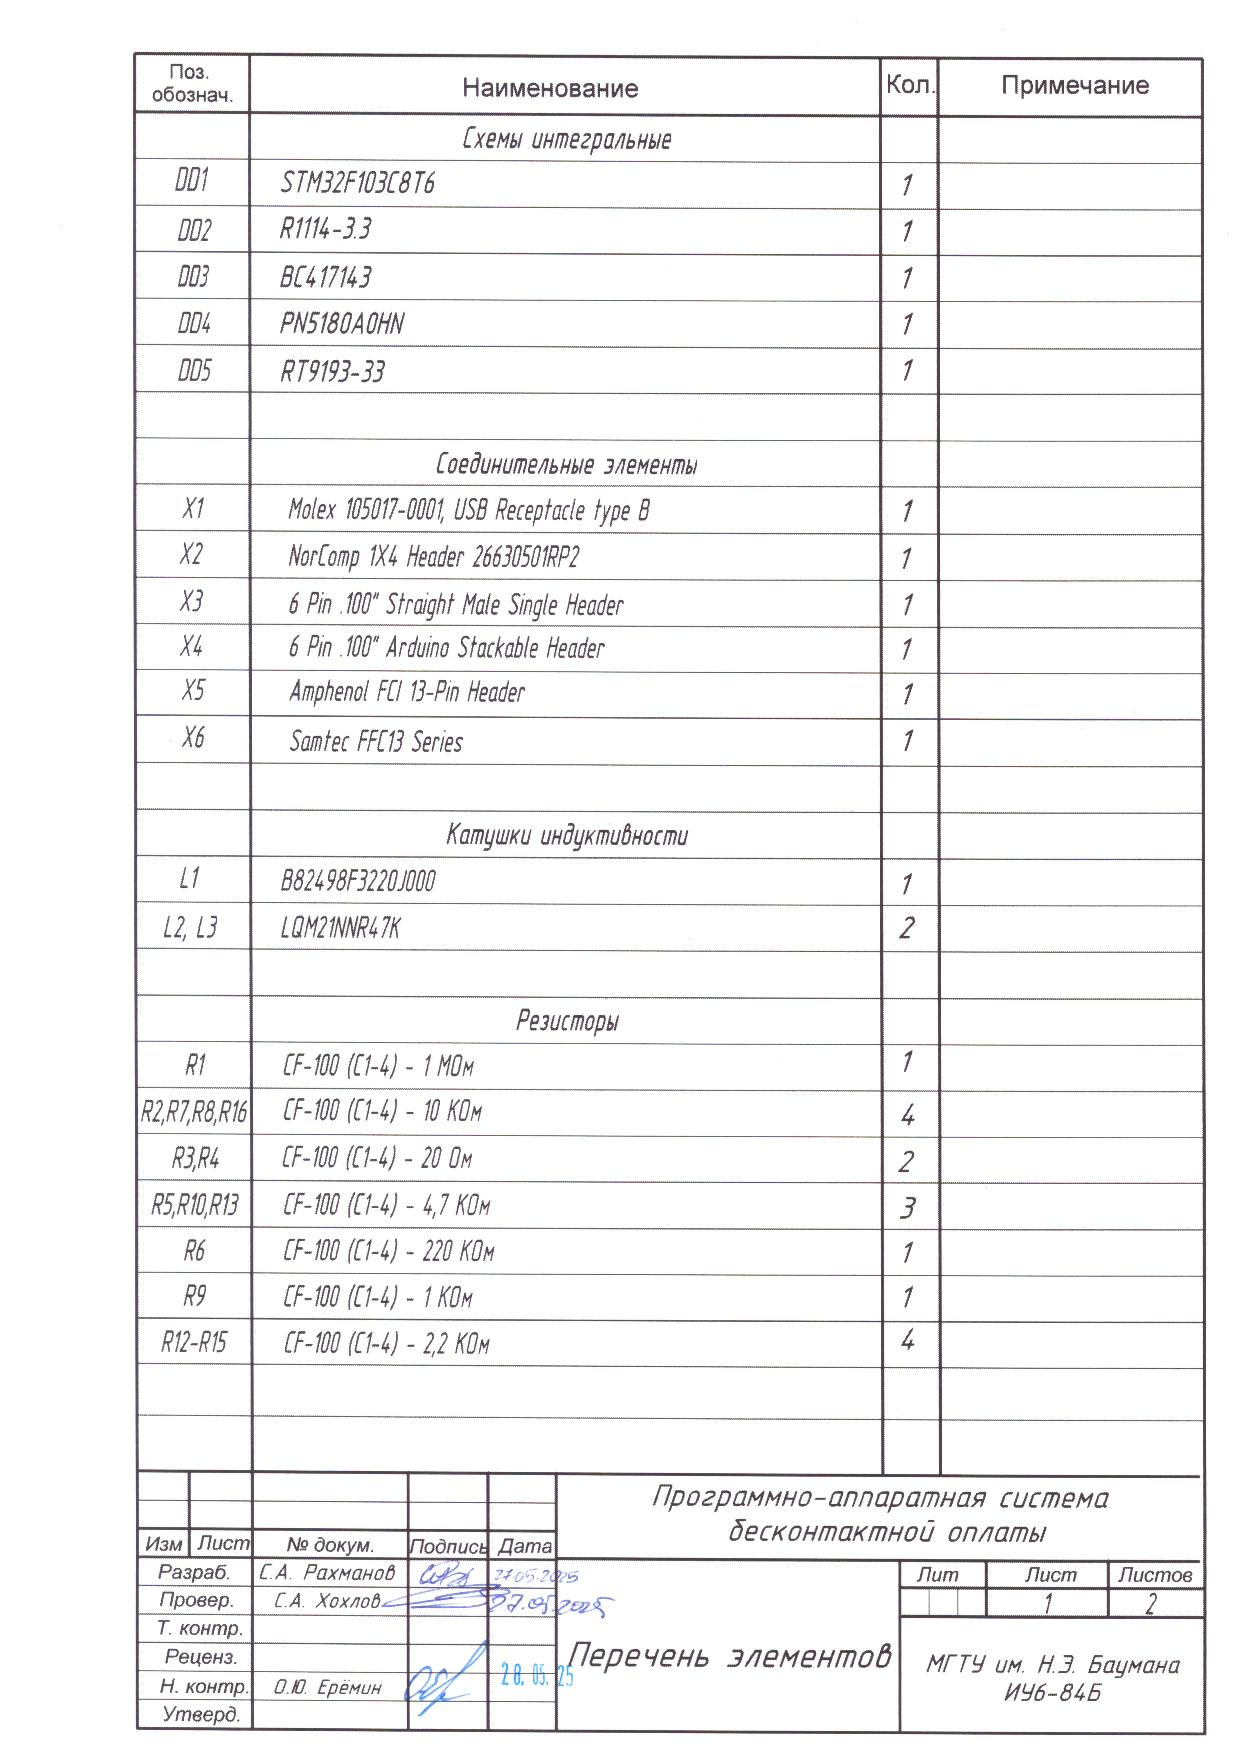
\includepdf[pages=1-2]{appendices/podpis/elements.pdf}
}{
    \setcounter{figure}{0}
    \renewcommand{\thefigure}{\Asbuk{appendixNum}\arabic{figure}}

    \begin{figure}[H]
        \centering
        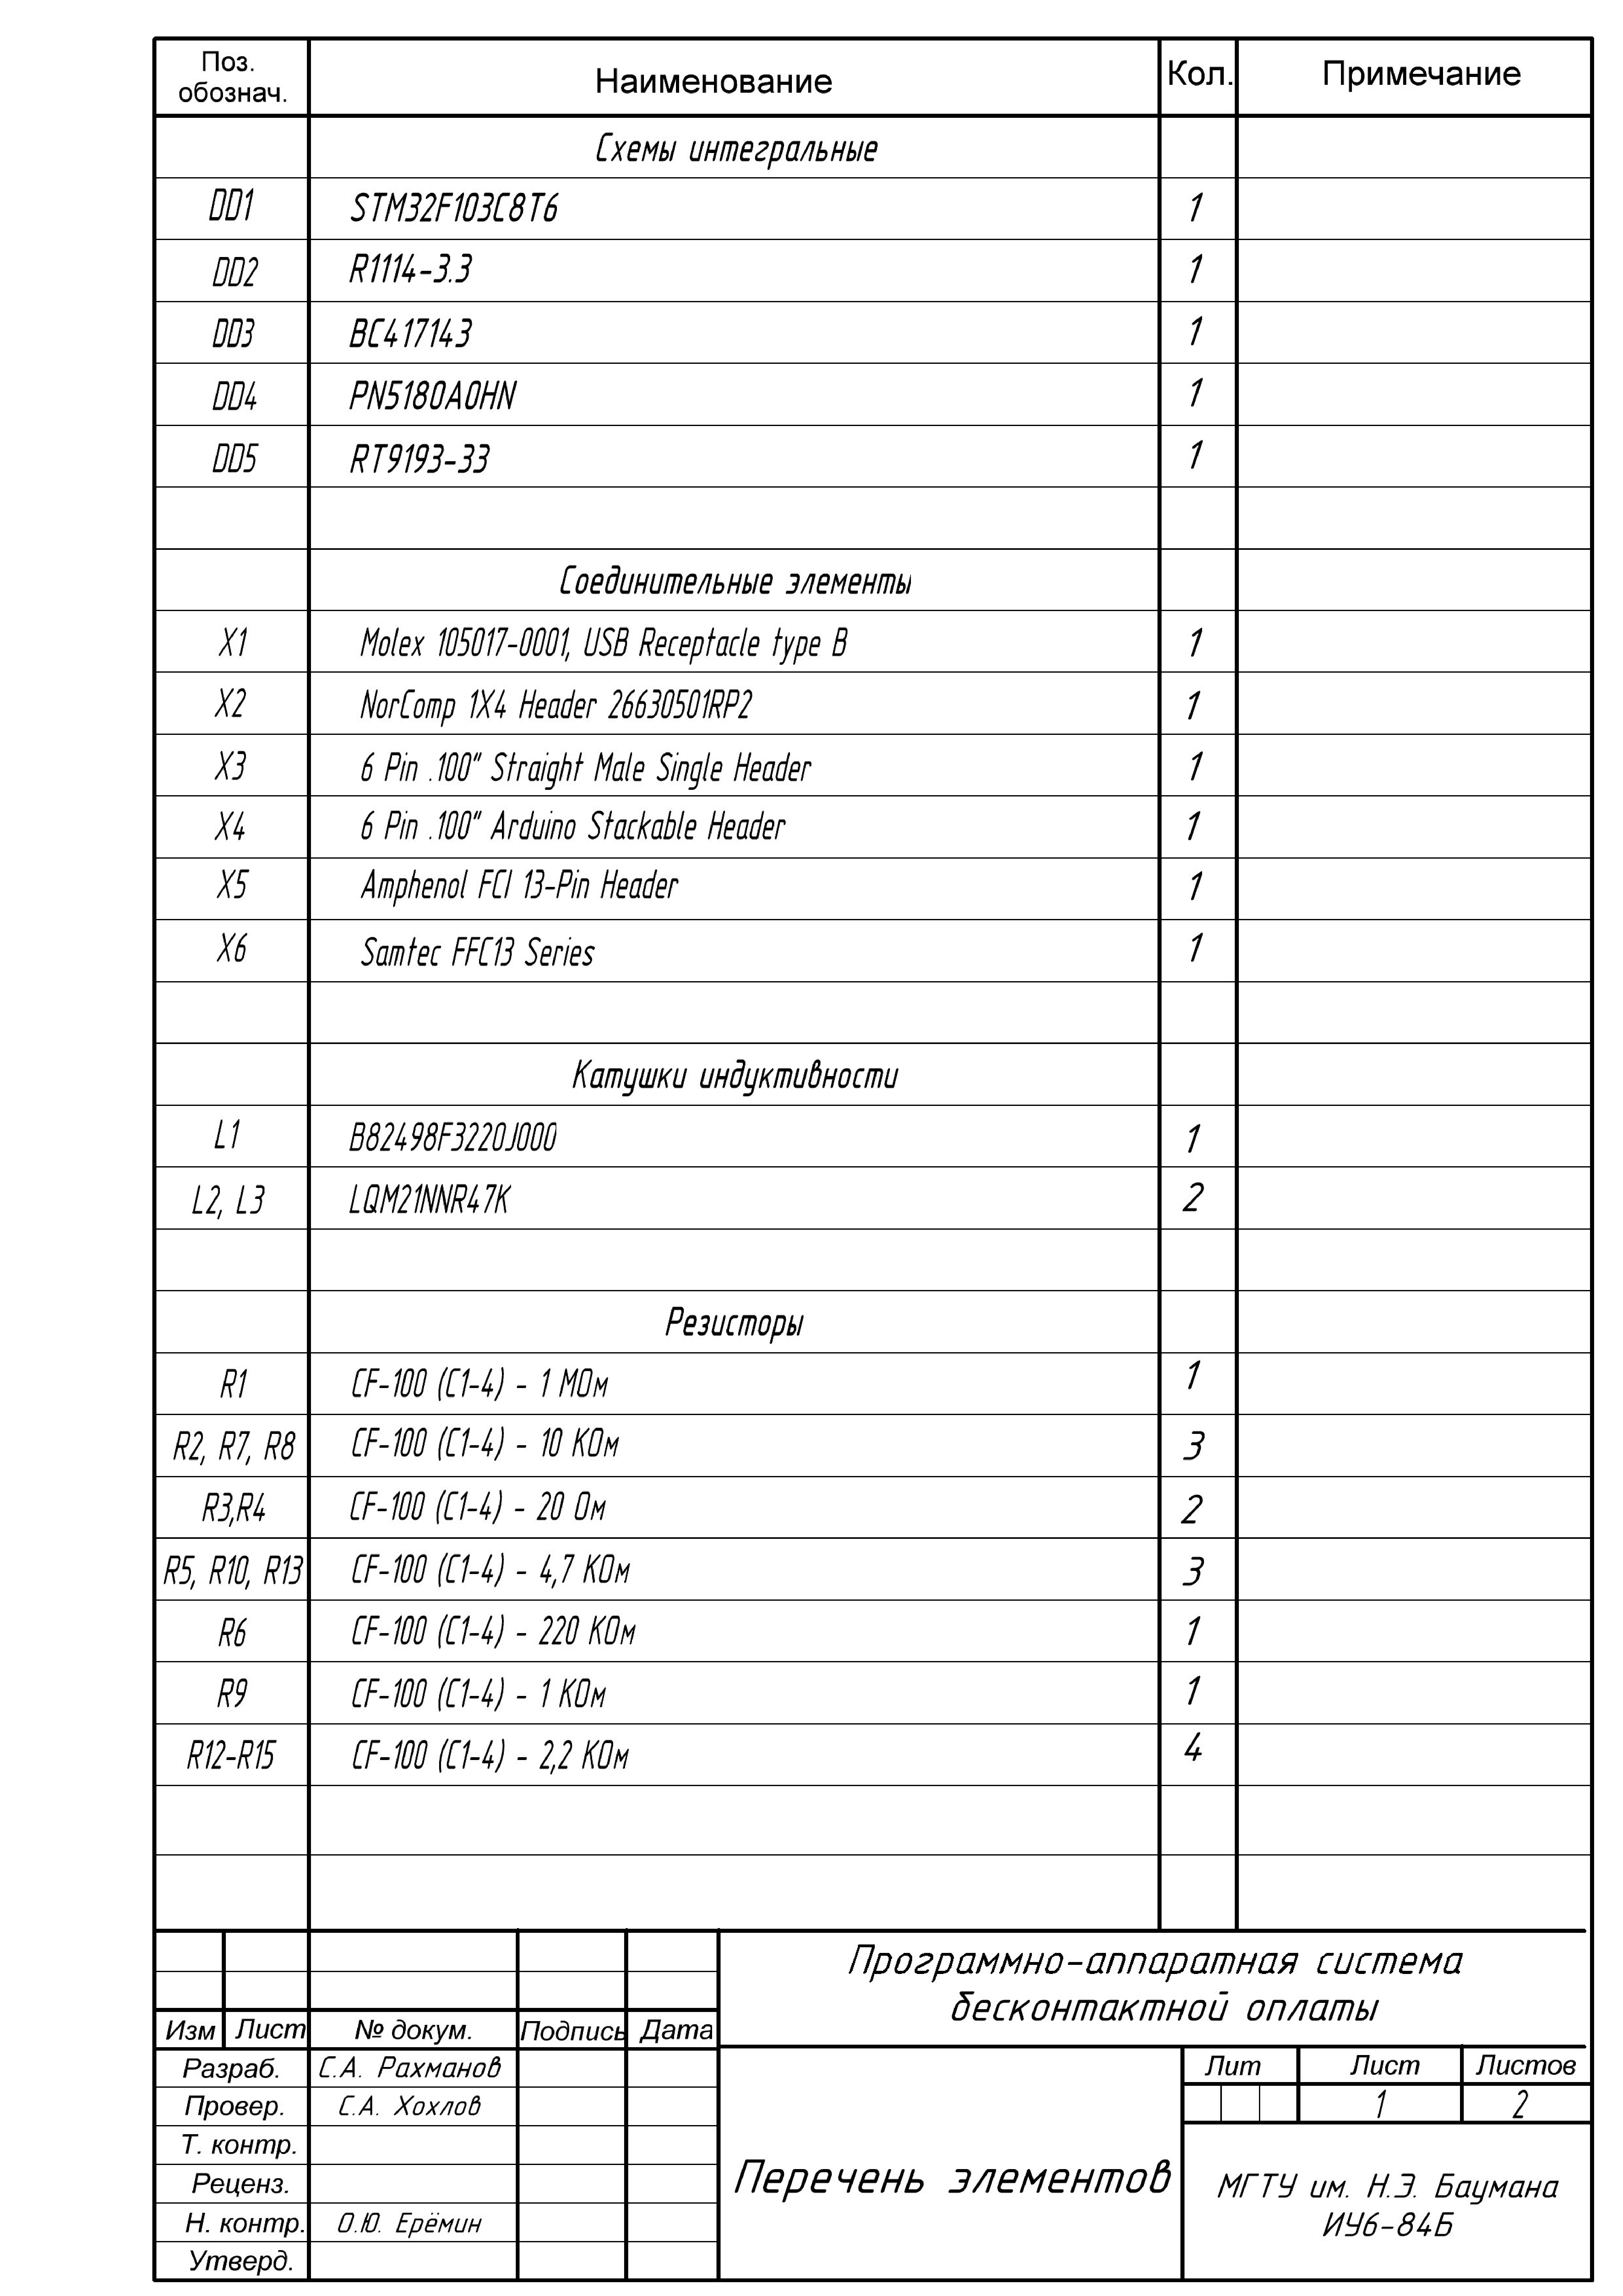
\includegraphics[height=0.95\textheight]{appendices/Спецификация Лист 1.jpg}
        \caption{Перечень элементов аппаратной части системы}
    \end{figure}

    \begin{figure}[H]
        \centering
        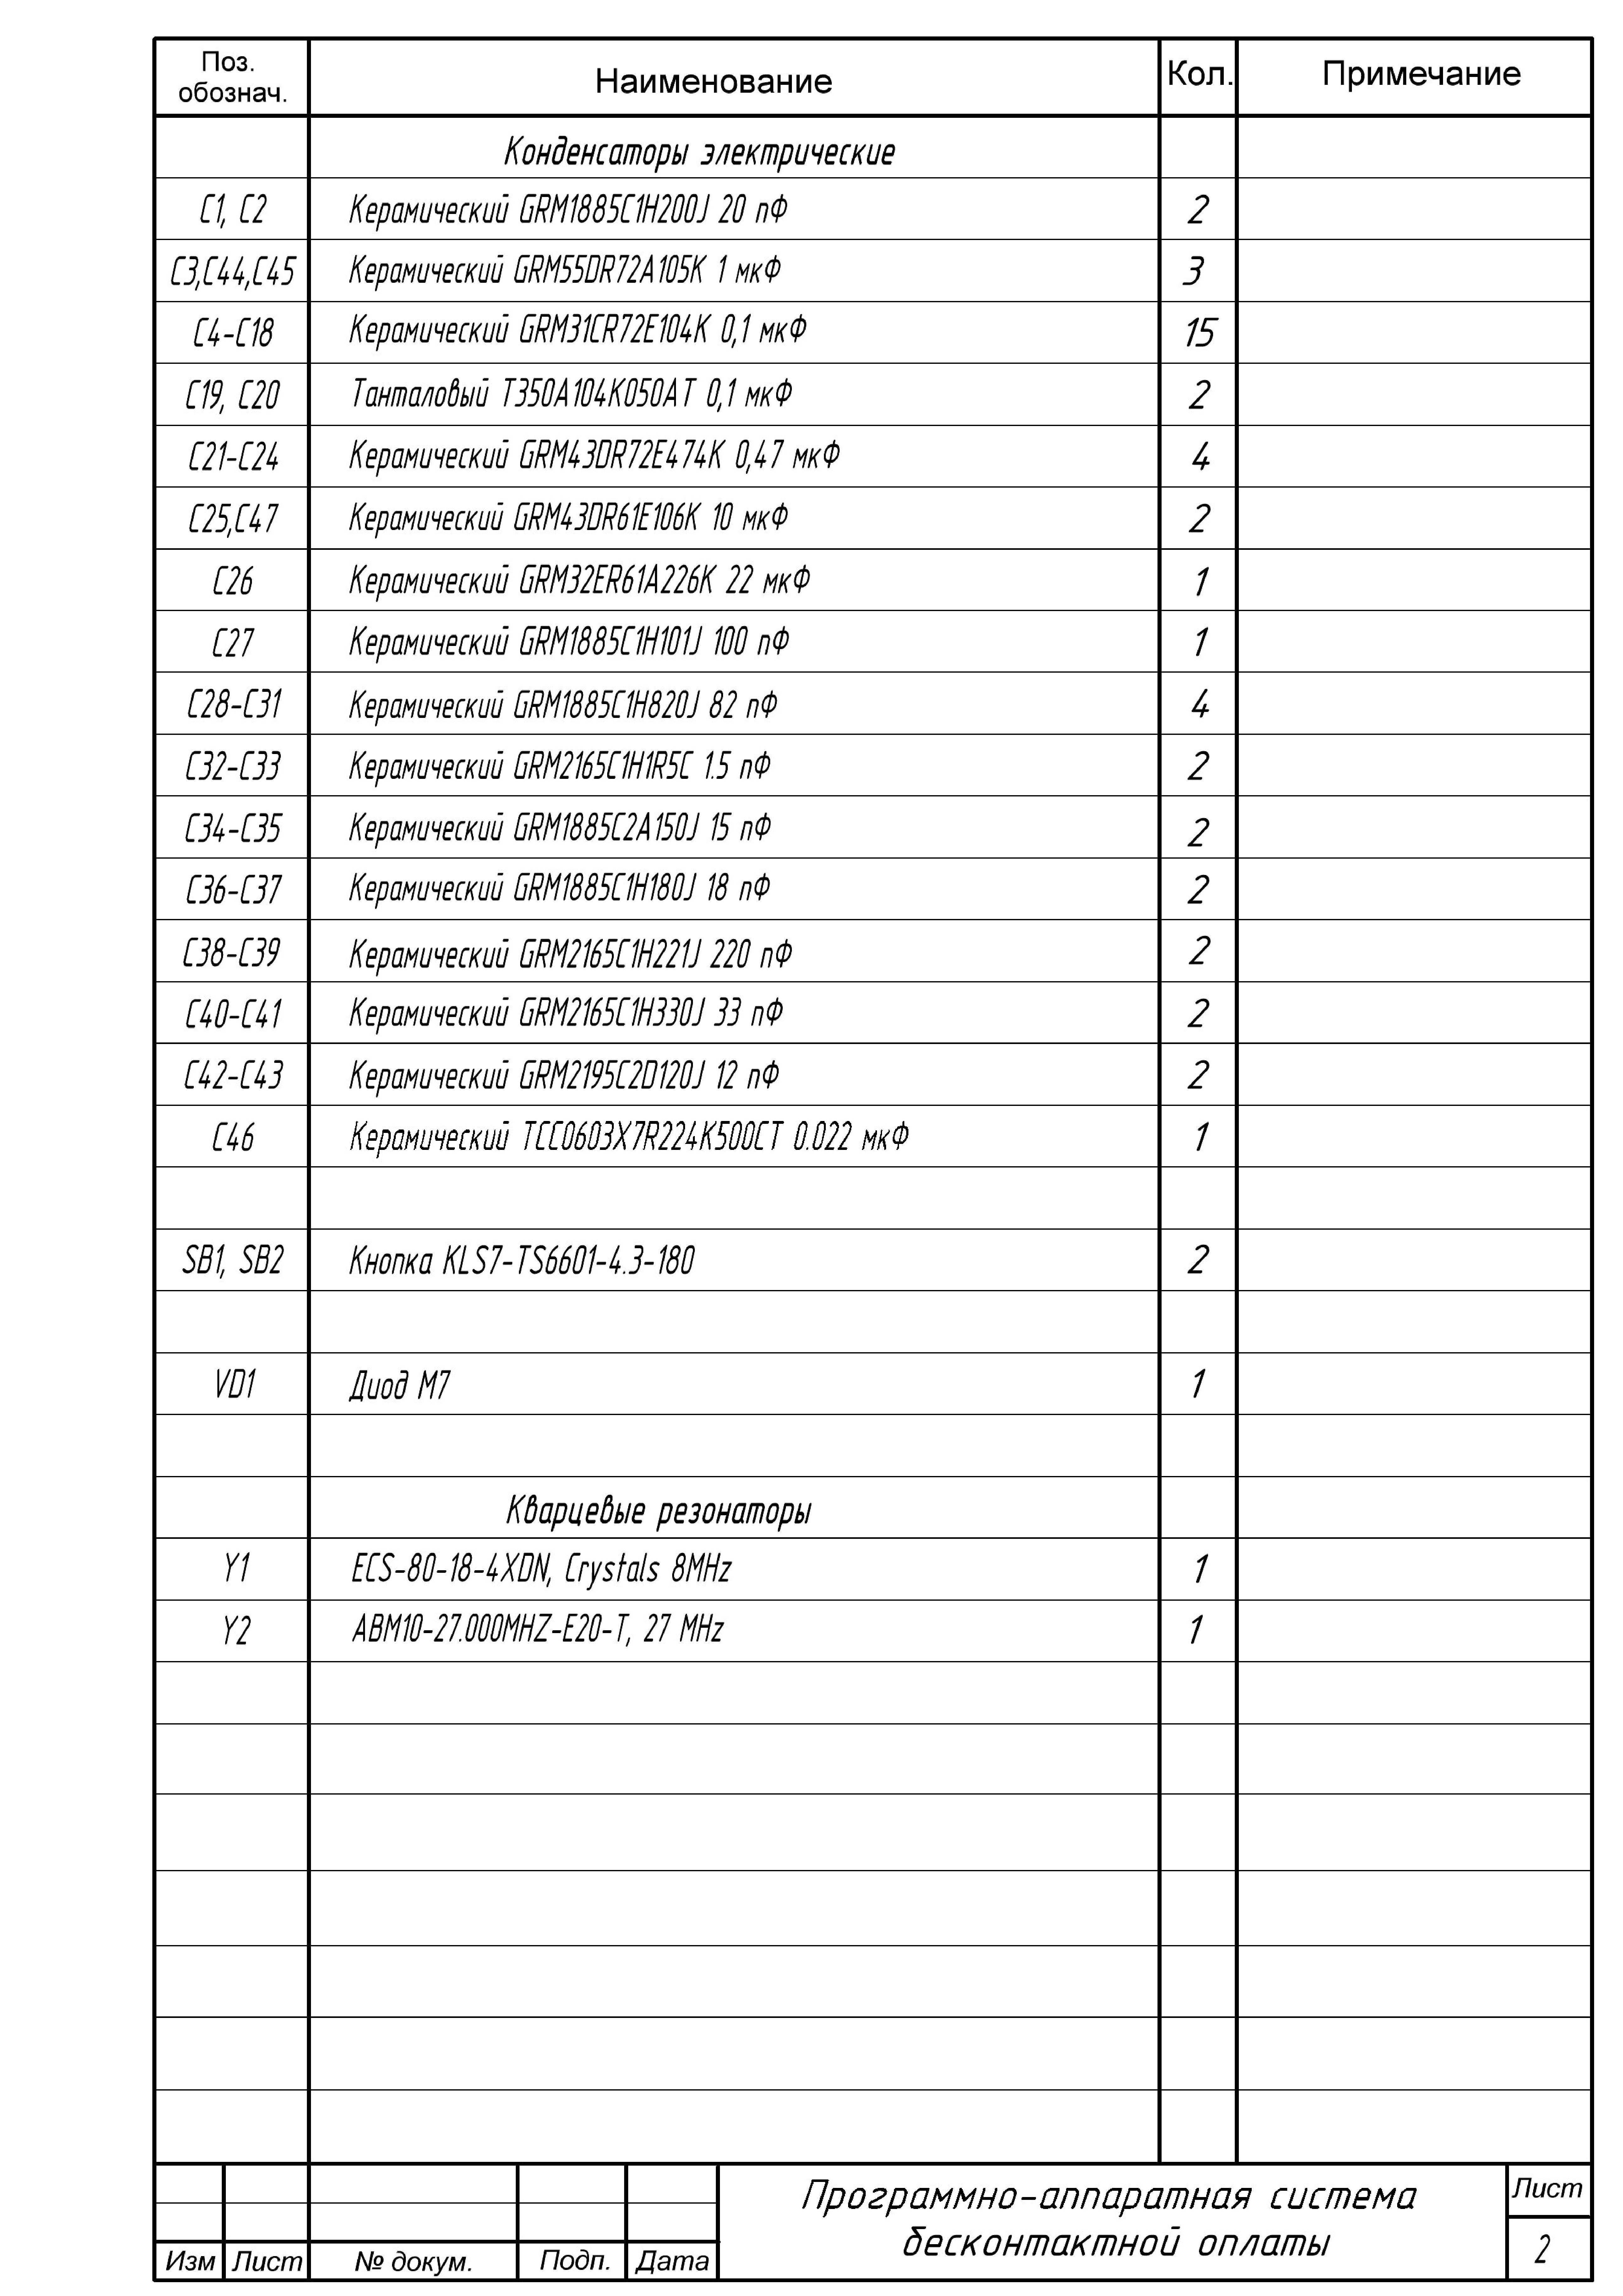
\includegraphics[height=0.95\textheight]{appendices/Спецификация Лист 2.jpg}
        \caption{Перечень элементов аппаратной части системы (окончание)}
    \end{figure}
}


% \addtocounter{page}{2}
